% (c) GreenSocs Ltd
% author: Christian Schroeder <schroeder@eis.cs.tu-bs.de>

%\documentclass[a4paper,12pt]{scrartcl}
\documentclass[a4paper,12pt,oneside]{gsbook}

\usepackage[utf8]{inputenc}

\usepackage{helvet}

\usepackage{hyperref}

\usepackage{greensocs}

\usepackage{graphicx}

\usepackage{multicol}

\usepackage{fancyhdr}

\usepackage{multirow}

\usepackage{tabularx}

\usepackage[dvips]{rotating} 

%% Christian's package CS_inputs
%\usepackage{verbatimfiles}
%\usepackage[outline,light]{draftcopy}

%\usepackage{ngerman}					% Regeln und Definitionen fuer deutschen Sprachraum
%\usepackage[latin1]{inputenc} % Umlaute
%\usepackage[T1]{fontenc}      % Woerter mit Umlauten richtig trennen
%\usepackage{ae}%um Einbindung von Type1-Fonts in PDF zu ermoeglichen
\usepackage{amsmath}						% Mathematik, fuer \text innerhalb $ $
%\usepackage[pdftex]{graphicx}
\usepackage{pifont} % needed for \ding{110} etc. (see new items)

\usepackage{lscape}			% ermoeglicht Querformat-Seiten, zwischen \begin{landscape} \end{landscape}

\usepackage{enumerate}	% ermoeglicht enumerate-Umgebung mit Option zu veraendern

\usepackage{listings}   % Listing von Programmcode
\lstloadlanguages{C}		% laedt die Regeln fuer Programmiersprache C
\usepackage{marvosym}		% fuer \lstset prebreak={\Righttorque} (Pfeil beim Umbruch einer Zeile)
\lstset{% general command to set parameter(s)
	basicstyle=\normalsize\ttfamily, % print whole listing
	stringstyle=\ttfamily, % typewriter type for strings
	keywordstyle=\ttfamily,
	showstringspaces=false,
	language=C,
	breaklines=true
}
\usepackage{color}			% fuer die Farbe der comments
\definecolor{keywordblue}{RGB}{0,0,255}
\definecolor{commentgreen}{RGB}{0,128,0}

\usepackage{float}
\restylefloat{table} % sorgt dafuer, dass [H] dafuer sorgt, dass Tabelle GENAU da ist, wo sie steht
\restylefloat{figure} % sorgt dafuer, dass [H] dafuer sorgt, dass figure GENAU da ist, wo sie steht
\usepackage{array}   % ermoeglicht komplexere Tabellen, vor allem mit automatischem Umbruch innerhalb der Zellen

%\usepackage{scrpage2} % ermoeglicht eigene Kopf- und Fu�zeilen, gehoert zum KOMA
%\usepackage{thumbindices} %create chapter thumb index on outer right side of pages (only works correct for pdfs)
%\usepackage{chapterthumb}
%create chapter thumb index on outer right side of pages (only works correct for pdfs)
%\usepackage{thumb}
\usepackage{longtable}
\usepackage{multirow}

\usepackage{xspace}
\usepackage{fancybox}  % Schattierte oder sonstig besondere Rahmen
\definecolor{dunkelgrau}{gray}{0.55}
\definecolor{hellgrau}{gray}{0.9}
\definecolor{hellhellgrau}{gray}{0.92}
\definecolor{weiss}{gray}{1}
\definecolor{schwarz}{gray}{0}
\usepackage{hhline}
\usepackage{colortbl}  % ermoeglicht farbige Tabellen

% aus de-tex-faq 5.3.4
% verhindert Hurenkinder und Schusterjungen (einzelne Zeilen nach/vor Seitenumbruch)
%\clubpenalty = 10000                               % TODO: wohlueberlegt einsetzen!!
%\widowpenalty = 10000 \displaywidowpenalty = 10000 % TODO: wohlueberlegt einsetzen!!

% EIGENE MAKROS:

% %%% ZwischenUberschrift %%%
\setlength{\fboxrule}{0.05cm}
%\newcommand{\ZwischenUberschrift}[1]{\vspace*{3ex}\textsf{\bfseries{#1}}\\[2ex]}
\newcommand{\ZwischenUberschrift}[1]{\vspace*{3ex}
	\noindent % nicht einruecken
	\boxput{
		\makebox(0,0)
			{
				\fcolorbox{weiss}{hellgrau}{\parbox[b]{\textwidth}{~}}
			}
	}
	{\parbox[b]{\textwidth}{\hspace*{2em}\textsf{\bfseries{#1}}}
	{	}
	}\vspace*{1ex}
	\nopagebreak
}

% %%% Verzeichnis %%%
\newsavebox{\VerzeichnisBox}
\newcommand{\Verzeichnis}[1]
	{
			\savebox{\VerzeichnisBox}{
\includegraphics{csimages/verzeichnis.eps} \textsf{#1}}
			\usebox{\VerzeichnisBox}
	}
	
% %%% Datei %%%
\newsavebox{\DateiBox}
\newcommand{\Datei}[1]
	{
			\savebox{\DateiBox}{
\includegraphics{csimages/datei.eps} \textsf{#1}}
			\usebox{\DateiBox}
	}
\newcommand{\DateiNoImg}[1]
	{
			\textsf{#1}
	}

% %%% Menue %%%
\newcommand{\Menue}[1]{\textsc{#1}}
% %%% Button %%%
\newcommand{\Button}[1]{\textsc{#1}}
% %%% Eingabe %%%
\newcommand{\Eingabe}[1]{
	\fcolorbox{weiss}{schwarz}{\textcolor{weiss}{\ttfamily #1}}
}

\newcommand{\befehl}[1]{\protect\mbox{\textsf{\textbf{\footnotesize{#1}}}}}			% einheitliche Befehle meines Protokolls
\newcommand{\Ohm}{$ \Omega $\xspace}										% Ohm fuer die Stueckliste
\newcommand{\uF}{$ \mu \text{F} $\xspace}
\setlength{\fboxrule}{0.05cm} % Rahmenbreite fuer box
\newcommand{\Achtung}[1]{	
	\begin{samepage}
		\noindent % nicht einruecken
		\fcolorbox{dunkelgrau}{hellhellgrau}{\parbox[b]{12cm}{#1}}
	\end{samepage}
}
\newcommand{\Parameter}[1]{\textsc{#1}} % Fuers Protokoll

\renewcommand{\labelitemi}{\textcolor{dunkelgrau}{\ding{110}}} % neues Zeichen fuer Aufzaehlunsebene 1
\renewcommand{\labelitemii}{\textcolor{dunkelgrau}{\ding{108}}} % neues Zeichen fuer Aufzaehlunsebene 2
\renewcommand{\labelitemiii}{\textcolor{dunkelgrau}{$\bullet$}} % neues Zeichen fuer Aufzaehlunsebene 2

\usepackage{makeidx}

\makeindex % ermoeglicht das erzeugen von Idizes mit \index{eintrag} Dann mit Makeindex weiterverarbeiten

\newcommand{\Note}[3]{
	\vspace{.5cm}
	\begin{minipage}{15cm}
		\noindent % nicht einruecken
		\rule{\textwidth}{.3pt}
		\Datei{} \textbf{\textsf{#1}}
		
		\textbf{#2}		
		
		#3
		
		\noindent % nicht einruecken
		\rule{\textwidth}{.3pt}
	\end{minipage}
	\vspace{.5cm}
}

% %%% Warning %%%
\newsavebox{\WarningSymbolBox}
\newcommand{\WarningSymbol}[1]
	{
			\savebox{\WarningSymbolBox}{
\includegraphics[height=1.7ex]{csimages/warning.eps} #1}
			\usebox{\WarningSymbolBox}
	}


%\usepackage{xspace}

% Fuer \begin{landscape}
\usepackage{lscape}

% allows [H] in figure
\usepackage{float}
\restylefloat{figure}

%Inlcudes fuer mathematische Formeln
\usepackage{amsmath,amsthm,latexsym}
\usepackage{wasysym}

\sloppy % Verhindert uebervolle H-Boxen (aber groessere Spaces!)
\nonfrenchspacing % Abstand nach Satzende immer gleich gross

% Verhindern von Schusterjungen (club) und Hurenkindern (widow)
\clubpenalty=10000
\widowpenalty=10000
\displaywidowpenalty=10000 

% sets spacing between paragraphs
\parskip 7.2pt

% Farbe fuer listings
\usepackage{color}  
\definecolor{stringblue}{RGB}{0,0,255}
\definecolor{keywordred}{RGB}{160,0,0}
\definecolor{commentgreen}{RGB}{0,128,0}
% Symbole fuer Listing-Umbruch-Pfeil
\usepackage{marvosym} 
\newcommand{\linebreaksign}{\hbox{\space\Righttorque}} % marvosym S.28 symbols-letter.pdf
\usepackage{listings}
\lstset{
  language=C++,
  %basicstyle=\ttfamily,
  breaklines=true,
  captionpos=b,
  breakatwhitespace=true,% erlaubt line break nur bei einem whitespace
  aboveskip=15pt, % Abstand ueber einem Listing
  basicstyle=\ttfamily \small,
  %identifierstyle=\it,%\bf,
  commentstyle=\color{commentgreen} \ttfamily, % mach mich dunkler
  stringstyle=\color{stringblue} \ttfamily,
  keywordstyle=\color{keywordred},
  showstringspaces=false,
  numbers=left,
  numberstyle=\tiny,
  numberfirstline=true,
  firstnumber=1,
  stepnumber=5,
  numbersep=5pt,
  %prebreak=\mbox{\tiny$\linebreaksign$}, 
  prebreak=\Righttorque,
  frame=trbl, % Rahmen
  tabsize=2             % 2 spaces per tab
}

%\makeatletter
%\DeclareRobustCommand*\textsubscript[1]{%
%  \@textsubscript{\selectfont#1}}
%\def\@textsubscript#1{%
%  {\m@th\ensuremath{_{\mbox{\fontsize\sf@size\z@#1}}}}}
%\makeatother

\hypersetup{%
  plainpages=false,
  colorlinks,   % Ausschalten fuer Druckversion
  linkcolor=blue,
  bookmarksnumbered,
  pdftitle={GreenReg User's Guide},
  pdfsubject={User's Guide for the GreenSocs GreenReg Device Register Framework},
  pdfauthor={Christian Schroeder, Technical University of Braunschweig, Dept. E.I.S. and GreenSocs Ltd},
  pdfkeywords={SystemC GreenSocs GreenReg DRF register},
  pdfstartview=FitH
}
\author{Copyright GreenSocs Ltd 2008\\ \\Developed by\\Christian Schr\"oder\\Technical University of Braunschweig, Dept. E.I.S.\\ \\ Based on Intel DRF}
\title{GreenReg User's Guide\\(GreenReg v.4.0.x)}% working draft)}

\renewcommand{\theenumi}{\arabic{enumi}}
\renewcommand{\theenumii}{\arabic{enumi}.\arabic{enumii}}
\renewcommand{\theenumiii}{\arabic{enumi}.\arabic{enumii}.\arabic{enumiii}}
\renewcommand{\theenumiv}{\arabic{enumi}.\arabic{enumii}.\arabic{enumiii}.\arabic{enumiv}}

% with subsubsections in tableofcontents
\setcounter{secnumdepth}{3}
\setcounter{tocdepth}{3}


%% new commands for this document
\newcommand{\GreenControl}{\mbox{\textsc{\small GreenControl}}\xspace}
\newcommand{\GreenConfig}{\mbox{\textsc{\small GreenConfig}}\xspace}
\newcommand{\GreenAV}{\mbox{\textsc{\small GreenAV}}\xspace}
\newcommand{\GreenReg}{\mbox{\textsc{\small GreenReg}}\xspace}
\newcommand{\DRF}{\mbox{\textsc{\small DRF}}\xspace}


\begin{document}

%Developed by Technical University of Braunschweig, Dept. E.I.S.
%Christian Schroeder
\maketitle

\tableofcontents
\enlargethispage{\baselineskip} % TODO: remove

% section Introduction
% (c) GreenSocs Ltd
% author: Christian Schroeder <schroeder@eis.cs.tu-bs.de>

\cleardoublepage
\chapter{Introduction}

The \GreenReg project\footnote{\GreenReg project page:  \href{http://www.greensocs.com/projects/GreenReg}{http://www.greensocs.com/projects/GreenReg}} provides a library that can be used for device and register modeling in ESL design. The project is based on the Intel \DRF framework.

\GreenReg can be understood as two parts: One side is the device and register modeling in the user model which is done by using the Device Register Framework (\DRF) API, the other is the configuration mechanism which is provided by \GreenConfig\footnote{\GreenConfig project page:  \href{http://www.greensocs.com/projects/GreenControl/GreenConfig}{http://www.greensocs.com/projects/GreenControl/GreenConfig}} and gives configuration tool access to the \DRF objects.

This allows ESL modelers to use the powerful configuration abilities of \GreenConfig to configure the \DRF objects.

The \GreenReg framework is not only a register framework. The way the user is able to model hardware registers and use their notifications for modeling behavior is a small model of computation.

%%%%%%%%%%%%%%%%%%%%%%%%%%%%%%%
\section{Further Reading}

This User's Guide focuses on the configuration aspect of \GreenReg and some enhancements to DRF.

See the \GreenReg Tutorial Slides\footnote{\hypertarget{lnk:TutorialSlides}{\GreenReg Tutorial Slides}:  \href{http://www.greensocs.com/Projects/GreenReg/docs/GreenRegTutorial}{http://www.greensocs.com/Projects/GreenReg/docs/GreenRegTutorial}} for more basic usage information and an introduction to the device and register modeling part. 


% section Implementation
% (c) GreenSocs Ltd
% author: Christian Schroeder <schroeder@eis.cs.tu-bs.de>

\cleardoublepage
\chapter{GreenReg}
\label{GreenReg}

This chapter guides through the enhancements of \GreenReg made to \DRF.

Section \ref{sec:NamespaceAndNamingConventions} clarifies some conventions used in this document and the code. Section \ref{sec:ConceptsAndBackground} shows some background information whereas sections \ref{sec:ModelingStyleWithFunctionsAndNotificationRules} and \ref{sec:WriteMask} are important sections telling how to use the \GreenReg enhancements. Section \ref{sec:ExpandingGreenReg} is for developers enhancing \GreenReg itself. The Notes section \ref{sec:Notes} notes general \GreenReg facts and small features, section \ref{sec:ImplementationCode} points to the code.

%%%%%%%%%%%%%%%%%%%%%%%%%%%%%%%
\section{Namespace and naming conventions}
\label{sec:NamespaceAndNamingConventions}
The \DRF classes of \GreenReg are located within the namespace {\sffamily gs::reg} and {\sffamily gs::reg\_utils}. Some configuration specific classes are in the namespace {\sffamily gs}.

For the correct namespace of the classes used in this document please
refer to the doxygen generated API reference.

The \GreenReg classes use some abbreviations (prefixes):
\begin{itemize}
	\item \emph{I\_} stands for {\em Interface}.
%	\item \emph{dr\_} stands for {\em \DRF user class}. falsch!
\end{itemize}

\paragraph{SystemC delimiter} The \GreenReg framework is developed using the dot ({\sffamily .}) as the SystemC delimiter within names, which follows the standard. Contrary to \GreenControl, \GreenReg does not allow to change this delimiter.

\paragraph{GreenReg specific report macros}
The end user should never use the internal \GreenReg report macros like \lstinline|GR_ERROR|, \lstinline|GR_REPORT_ERROR| etc!


%%%%%%%%%%%%%%%%%%%%%%%%%%%%%%%
%\section{Quick Start}



%%%%%%%%%%%%%%%%%%%%%%%%%%%%%%%
\section{Concepts and Background}
\label{sec:ConceptsAndBackground}



%%%%%%%%%%%%%%%%%%
\subsection{Register accesses}

There are two basic \GreenReg ways accessing registers:
\begin{enumerate}
	\item Access the register directly from within the register or using the register container
	\item Access the register from the bus
\end{enumerate}
If the register makes a difference between its in and out buffers (e.g. a splitio register) it is important to know the behavior the different accesses:

\noindent
\begin{tabular}[z]{|p{4cm}|p{5cm}|p{7cm}|}
	\hline
	\textsl{Way of access} & \textsl{Accessed buffer} & \textsl{Example} \\ 
	\hline
	\hline
	set function \newline(and operator =) \newline Parameter access & write {\em out buffer} & \lstinline|r[0x01] = 5;| \\
	\hline
	get function & read {\em in buffer} & \lstinline|unsigned int val = r[0x01];|\\
	\hline
	bus write & write {\em in buffer} & \lstinline|m_master_port->write(0x01, dat, 4);| \newline \lstinline|r.bus_write(data, 0x01, offset);| \\
	\hline
	bus read & read {\em out buffer} & \lstinline|cr = m_master_port->read(0x01, 4);| \newline \lstinline|r.bus_read(data, 0x01, offset);|\\
	\hline
\end{tabular}

The references {\sffamily i} and {\sffamily o} of class {\sffamily I\_register} can be used to access the buffers explicitly.


%%%%%%%%%%%%%%%%%%
\subsection{Types of configuration utilization}
\label{sec:TypesConfigUtils}
\GreenReg internally uses two different ways of connecting \GreenReg data types to the \GreenConfig framework to provide the \GreenReg data types as configurable parameters:
\begin{enumerate}
  \item {\bf The internal \GreenReg data storage {\em is} a \GreenConfig parameter.} \newline
  This is like it's done for {\sffamily dr\_attribute}. This needs no further \GreenReg specific explanation. See the \GreenConfig User's Guide how to use parameters.
  \item {\bf The parameter API is implemented by the \GreenReg data type to {\em make} it a parameter.} \newline
  For a guide how to make use of the {\sffamily gs\_param\_drf}-adapter see section \ref{sec:HowToUtilizeParameters}.
\end{enumerate}



%%%%%%%%%%%%%%%%%%%%%%%%%%%%%%%
\section{Modeling Style with Functions and Notification Rules}
\label{sec:ModelingStyleWithFunctionsAndNotificationRules}

This section is about how to model registers and the dependent methods or functions with GreenReg.

The basic modeling concept is that you have registers which can be equipped with different kinds of methods (like SC\_METHODs) or more efficient functions (GR\_FUNCTIONs) to react on register changes.

The procedure is the following:\vspace{-1em}
\begin{itemize}
  \item Create a register  \vspace{-.5em}
  \item Announce a method/function (and implement it) \vspace{-.5em}
  \item Create a notification rule the method/function is sensitive to and which defines under which conditions the method /function will be notified/called (possibly delayed).
\end{itemize}

%%%%%%%
\subsection{Methods/functions and their Characteristics}

The different methods being available for notification rule notification / callbacks are:
\begin{itemize}
  \item {\sffamily GR\_FUNCTION}  \vspace{-.5em}
  \item {\sffamily GR\_FUNCTION\_PARAMS}  \vspace{-.5em}
  \item {\sffamily GR\_METHOD} {\em (not recommended)}
  \item {\sffamily SC\_METHOD} {\em (not recommended)}
\end{itemize}

Please report to the author(s) of this document which methods/functions you use most and which ones are needless in your opinion.


%%%
\paragraph{GR\_FUNCTION} \addcontentsline{toc}{subsubsection}{GR\_FUNCTION}
A {\sffamily GR\_FUNCTION} is an equivalent to the SystemC {\sffamily SC\_METHOD} with the difference that it is activated by a {\sffamily gr\_event} by callback, not by an {\sffamily sc\_event} notify. This can either happen immediately, with an {\sffamily SC\_ZERO\_TIME} delay (like usual {\sffamily sc\_event}s behave) or with another delay, see the different sensitive macros (\ref{sec:sensitivity}) and the socket-wide delay switch (\ref{sec:DelayedSwitch}).

\WarningSymbol{}{A {\sffamily GR\_FUNCTION} does not need (and even cannot handle) a {\sffamily dont\_initialize()} call.}

\WarningSymbol{}{ A {\sffamily GR\_FUNCTION} is not allowed to use SystemC {\sffamily SC\_METHOD} or {\sffamily SC\_THREAD} specific elements because the function is called by the callback in (potentially) any SystemC context.}

For the callback register any void-void function with the following signature using the {\sffamily GR\_FUNCTION} macro:\vspace{-.5em}
\begin{lstlisting}
GR_FUNCTION(class_name, function_name); 
// will be concatenated to &class_name::function_name
// which needs to be of type callback_type
typedef void(class_name::*callback_type)()

// e.g.

void function_name();
\end{lstlisting}

Example (stripped-down):
\begin{lstlisting}
void end_of_elaboration() {
  GR_FUNCTION(UserDevice, gr_function_callback);
  GR_SENSITIVE(r[0x01].add_rule(gs::reg::POST_WRITE, "pw1", [...]));
}
void gr_function_callback() {
  cout << "got not delayed post write notification for Reg 0x01" << endl;
}
\end{lstlisting}

%%%
\paragraph{GR\_FUNCTION\_PARAMS} \addcontentsline{toc}{subsubsection}{GR\_FUNCTION\_PARAMS}
A {\sffamily GR\_FUNCTION\_PARAMS} enhances the {\sffamily GR\_FUNCTION} with arguments. When being called, the callback function gets the transaction which caused the register access (if there was a bus access, otherwise it will get NULL) and the delay the function call had been delayed (if it had been delayed, otherwise it will get {\sffamily SC\_ZERO\_TIME}).

\WarningSymbol{Remark:}{The called function is not able to distinguish between an immediate (not delayed) call and a zero time (delta cycle) delayed call. 
\newline TODO: The function could get another (bool) parameter showing if the call had been delayed.}

\WarningSymbol{}{A {\sffamily GR\_FUNCTION\_PARAMS} does not need (and even cannot handle) a {\sffamily dont\_initialize()} call.}

\WarningSymbol{}{A {\sffamily GR\_FUNCTION\_PARAMS} is not allowed to use SystemC {\sffamily SC\_METHOD} or {\sffamily SC\_THREAD} specific elements because the function is called by the callback in (potentially) any SystemC context.}

For the callback register a function with the following signature using the {\sffamily GR\_FUNCTION\_PARAMS} macro: \vspace{-.5em}
\begin{lstlisting}
GR_FUNCTION_PARAMS(class_name, function_name); 
// will be concatenated to &class_name::function_name
// which needs to be of type callback_type
typedef void(class_name::*callback_type)(gs::reg::transaction_type*&, const sc_core::sc_time&)

// e.g.

void function_name(gs::reg::transaction_type* &tr, 
                   const sc_core::sc_time& delay);
\end{lstlisting}

Example (stripped-down):
\begin{lstlisting}
void end_of_elaboration() {
  GR_FUNCTION_PARAMS(UserDevice, gr_function_callback_p);
  GR_SENSITIVE(r[0x01].add_rule(gs::reg::POST_WRITE, "pw1", [...]));
}
void  gr_function_callback_p(gs::reg::transaction_type* &tr, const sc_core::sc_time& delay) {
  cout << "got not delayed post write notification for Reg 0x01 with params" << endl  << "transaction ID = " << tr->getTransID());
}
\end{lstlisting}


%%%
\paragraph{GR\_METHOD} \addcontentsline{toc}{subsubsection}{GR\_METHOD}
A {\sffamily GR\_METHOD} is a {\sffamily GR\_FUNCTION} which is additionally an {\sffamily SC\_METHOD} internally. It should only be used if special features of the SystemC method are needed. 

\WarningSymbol{}{A {\sffamily GR\_METHOD} {\em does handle} the {\sffamily dont\_initialize()} call. You need to use it to avoid activation during initialization. }

\WarningSymbol{}{ A {\sffamily GR\_METHOD} is not allowed to use SystemC {\sffamily SC\_METHOD} or {\sffamily SC\_THREAD} specific elements because the function is called by the callback in (potentially) any context.}

Example (stripped-down):
\begin{lstlisting}
void end_of_elaboration() {
  GR_METHOD(UserDevice, gr_method_notification);
  GR_SENSITIVE(r[0x01].add_rule(gs::reg::POST_WRITE, "pw1", [...]));
  dont_initialize();
}
void gr_method_notification() {
  cout << "got post write notification (callback or notify) for Reg 0x01" << endl;
}
\end{lstlisting}


The three {\sffamily GR\_} functions/methods all use callbacks to call the user-registered function. This happens either immediately (efficient!) or delayed by an internal payload event queue (inefficient as SystemC methods but with payload if desired).

\Note{Implementation Details}{Why {\sffamily GR\_FUNCTION / METHOD}s?}{
The {\sffamily GR\_FUNCTION}s have been introduced due to performance reasons:
The default SystemC way is to use {\sffamily SC\_METHOD}s which are triggered by {\sffamily sc\_event}s. Events are the worst thing for performance because the SystemC kernel needs to do a context switch. The idea of {\sffamily GR\_METHOD}s is using simple callbacks (that's why the macro needs the class name) without the need of the context switch.\newline 
This has the disadvantage that you do not know in which context the method is called (may be {\sffamily SC\_METHOD}, an {\sffamily SC\_THREAD},...). Accordingly you are not allowed to use specific {\sffamily SC\_METHOD} calls like {\sffamily next\_trigger()}. We cannot bypass this issue following the standard.
}

%%%
\paragraph{SC\_METHOD} \addcontentsline{toc}{subsubsection}{SC\_METHOD} 
An {\sffamily SC\_METHOD} should only be used if special features of the SystemC method are needed.

\WarningSymbol{}{Of course handles an {\sffamily SC\_METHOD} the {\sffamily dont\_initialize()} call.}

When using {\sffamily SC\_METHOD}s you need to enable the notify within the {\sffamily gr\_event} - which may be disabled by default. See section \ref{sec:EventNotificationRules} how to use {\sffamily SC\_METHOD}s with event notification rules and for event switch details see section \ref{sec:EventSwitch}.


%%%%%%%
\subsection{Sensitivity}
\label{sec:sensitivity}

The three different methods/functions are used in combination with a sensitivity statement: \vspace{-1em}
\begin{itemize}
  \item {\sffamily SC\_METHOD}s use the standard SystemC \lstinline|sensitive << notification_rule_event;| \newline
  whereas
  \item {\sffamily GR\_FUNCTION}s and {\sffamily GR\_FUNCTION\_PARAMS} can use either 
    \begin{itemize}
      \item {\sffamily GR\_SENSITIVE(notification\_rule\_event);} or 
      \item {\sffamily GR\_DELAYED\_SENSITIVE(notification\_rule\_event, delay\_time);}, 
    \end{itemize}
   see examples and details below.
\end{itemize}

\paragraph{SystemC sensitivity for {\sffamily SC\_METHOD}s}
It is possible (but not recommended) to use the notification rule's {\sffamily gr\_event} as an input for the usual SystemC {\sffamily SC\_METHOD} sensitivity. See sections \ref{sec:EventNotificationRules} and \ref{sec:EventSwitch} how to use the event switch.

\paragraph{{\sffamily GR\_SENSITIVE}} The macro {\sffamily GR\_SENSITIVE} can be used as a replacement just like the standard sensitive statement. The notification rule's {\sffamily gr\_event} will make an immediate callback to the {\sffamily GR\_FUNCTION} (or {\sffamily GR\_FUNCTION\_PARAMS}) when the notification rule condition matches. 

This callback is independent from the event switch (sec. \ref{sec:EventSwitch})!

\noindent
\begin{minipage}{\textwidth}
Macro syntax:
\vspace{-1ex}
\begin{lstlisting}
GR_SENSITIVE(notification_rule);
\end{lstlisting}
\end{minipage}

\paragraph{{\sffamily GR\_DELAYED\_SENSITIVE}} The macro {\sffamily GR\_DELAYED\_SENSITIVE} causes a callback similar to the previous one but can delay this callback. The macro gets an additional time parameter which defines the time the callback should be delayed. If the delay is applied can be switched on and off with the {\em delayed switch} (sec. \ref{sec:DelayedSwitch}).

This callback is independent from the event switch (sec. \ref{sec:EventSwitch})!

\WarningSymbol{Remark:}{By default (only) all bus accesses are delayed with the delay time specified in the macro. Direct local access notifications are not delayed. Hence the delayed sensitivity should only be used for bus access notifications. Local accesses to {\sffamily bus\_read} and {\sffamily bus\_write} functions can be delayed by switching the according parameter to {\sffamily true}.}

\noindent
\begin{minipage}{\textwidth}
Macro syntax:
\vspace{-1ex} 
\begin{lstlisting}
GR_DELAYED_SENSITIVE(notification_rule, sc_time);
\end{lstlisting}
\end{minipage}

See the example \Verzeichnis{greenreg/examples/simple} for a complete example using different types of sensitivities and functions.

%%%%%%%
\subsection{Notification Rules and Callbacks}

This is only a short introduction to notification rules, what they are for and how to use them. See the \hyperlink{lnk:TutorialSlides}{Tutorial Slides} for more details. This section handles the configurability of notification rules (subsection \ref{sec:NotificationRuleConfiguration}) and the difference between event driven notification rules and callback driven ones (further subsections).

\Note{Implementation Details}{Notification rules}{
Notification rules are added by calling \lstinline|add_rule| on a register, attribute or bit\_range. This creates an \lstinline|I_notification_rule| (one of its implementations) which owns a \lstinline|dr_event|. This \lstinline|dr_event| is notified when a rule is processed. \newline
The \lstinline|dr_event| can be switched to use an \lstinline|sc_event| being notified {\em or} to use a callback.
}

There are two ways the user can get notifications / callbacks from registers. The concept is to keep the notification rules and configuration parameter callbacks separated.

\begin{itemize}
  \item Use {\em parameter callbacks} for configuration and analysis of your system but {\em not} for modeling.
  \item Use {\em notification rules} to model your system (they are highly configurable and provide special register features). \newline  Notification rules provide two ways of usage:
  \begin{itemize}
    \item Notification rules with events (default, see section \ref{sec:EventNotificationRules}):\newline
     When the rule is matched, the event which is returned by the \lstinline|add_rule()| call is fired. 
    \item Notification rules with callbacks (see section \ref{sec:CallbackNotificationRules}): \newline
     When the rule is matched, the registered callback is called instead of the event being fired. 
  \end{itemize}
\end{itemize}

%%%%%%%
\subsubsection{Configuration of Notification Rules}
\label{sec:NotificationRuleConfiguration}

See the \hyperlink{lnk:TutorialSlides}{Tutorial Slides} and further (not yet existing) documentation about how to specify notification rules.

%%%%%%%
\subsubsection{Event-based Notification Rules {\em (not recommended!)}}
\label{sec:EventNotificationRules}

Event-based notification rules are the default SystemC-like way using \lstinline|SC_METHOD|s being activated by events. The advantage of this way is that the behavior of notifications and method activations is very SystemC-like, so SystemC users get the behavior they expect. The drawback of this way is the lack of efficiency. The notification of the events consume simulation time as well as the {\sffamily wait} statements that are needed allowing pre- and post-notifications on each register change. If no hard requirements conflicts with callbacks, better use callback-based notification rules (see section \ref{sec:CallbackNotificationRules}). 

Whenever you use this way you should ensure the events are enabled by calling {\sffamily enable\_events()} for the register. For legacy code the events can be (are {\em for the current release}) enabled by default (see section \ref{sec:EventSwitch}).

Example usage: 

\noindent
\begin{minipage}{\textwidth}
\begin{lstlisting}
void end_of_elaboration() {
  SC_METHOD( show_notification_reg1_SC_M );
  sensitive << r[0x01].add_rule(GreenReg::USR_OUT_WRITE, "written_to_reg1", GreenReg::NOTIFY);
  dont_initialize();
  r[0x01].enable_events();
}
void show_notification_reg1_SC_M() {
  cout << sc_time_stamp() << "got register notification for Reg1" << endl;
  cout << "value = 0x" << hex << r[0x01] << dec << endl;
}
\end{lstlisting}
\end{minipage}

%%%%%%%
\subsubsection{Callback-based Notification Rules}
\label{sec:CallbackNotificationRules}

The more efficient way of modeling is using callback-based notification rules. They are used in conjunction with \lstinline|GR_FUNCTION|s which do not need kernel context switches and events being fired but uses direct efficient function calls. When having switched off events (see section \ref{sec:EventSwitch}), even the {\sffamily wait} in between the pre- and post-calls is omitted. 

See the following example how to use \lstinline|GR_FUNCTION|s. The macro needs the class the callback needs to be called and common the sc\_sensitive is replaced by a macro:
 
\noindent
\begin{minipage}{\textwidth}
\begin{lstlisting}
void end_of_elaboration() {
  GR_FUNCTION(MyMod, show_notification_reg1_GR_M);
  GR_SENSITIVE(r[0x01].add_rule( GreenReg::USR_OUT_WRITE, "written_to_reg1", GreenReg::NOTIFY));
  dont_initialize();
}
void show_notification_reg1_GR_M() {
  cout << "got register notification call for Reg1" << endl;
  cout << "value = 0x" << hex << r[0x01] << dec << endl;
}
\end{lstlisting}
\end{minipage}


%%%%%%%
\subsubsection{Delayed Switch}
\label{sec:DelayedSwitch}

The {\em delayed switch} activates and deactivates the delay of pre- and post- write and read notification rules being caused by bus accesses.

The delay activation is applied to the notification rule by the receiving socket (class \mbox{{\sffamily GSGPSOCKET::slave\_base})} on each received register access. Hence there is a switch in the slave socket that can be toggled to enable and disable the delay dynamically during simulation runtime. The switch will apply to all register accesses over this socket.

The interface is the following one:
\vspace{-1ex}
\begin{lstlisting}
/// Disables the delay 
/// for all notification rule callbacks caused by this socket
void disable_delay();
/// Enables the delay
/// for all notification rule callbacks caused by this socket
void enable_delay();
/// Returns if the delay is enabled
bool delay_enabled();
\end{lstlisting}

Example:
\vspace{-1ex}
\begin{lstlisting}
class ReceiverSlaveDevice 
: public gs::reg::gr_device 
{
public:
  // Slave socket with delayed switch
  gs::reg::greenreg_socket< GSGPSOCKET::generic_slave> m_slave_socket;
  
  GC_HAS_CALLBACKS();
  SC_HAS_PROCESS( ReceiverSlaveDevice );
	
  ReceiverSlaveDevice(sc_core::sc_module_name name) 
  : gr_device(name, gs::reg::INDEXED_ADDRESS, 2, NULL)
  , m_slave_spcket( "slave_socket", r, 0x0, 0xFFFFFFFF) // Slave socket
  { [...] }
  // SC_THREAD which demonstrates how the delayed switch can be switched
  void delayed_switch_demo() {
    wait(11, sc_core::SC_NS);
    m_slave_port.disable_delay();
    wait(10, sc_core::SC_NS);
    m_slave_port.enable_delay(); 
  }
}
\end{lstlisting}

%%%%%%%
\subsubsection{Order Notification Rules}
\label{sec:OrderNotificationRules}

In order to create dependencies between several notification rules there is the option to order the existing rules:

Notification rules are stored in an ordered vector (in the {\sffamily notification\_rule\_container}). The order can be manipulated using the functions \lstinline|move_rule_to_front| and \lstinline|move_rule_to_back| both moving the notification rule specified by name to the desired position.

Example:

\vspace{-1ex}
\noindent
\begin{minipage}{\textwidth}
\begin{lstlisting}
DR_METHOD(MyMod, show_notification_reg0_DR_1);
DR_SENSITIVE(r[0x00].add_rule(
  DRF::USR_OUT_WRITE, "written_to_reg0_DR_1", DRF::NOTIFY));
dont_initialize();

[...]

r[0x00].get_user_obuf_write_rules(). move_rule_to_back("written_to_reg0_DR_1");
\end{lstlisting}
\end{minipage}


%%%%%%%
\subsection{Use cases}
\label{sec:UseCases}

This section gives a short overview over some use cases and suggestions how to model.

\noindent
\begin{minipage}{\textwidth}
\ZwischenUberschrift{Efficient standard case}
{\bf Case:} Standard case: You want to model a more efficient {\sffamily SC\_METHOD}-like function without using inefficient events.\\
{\bf Suggestion:} Use an {\sffamily GR\_FUNCTION} with the {\sffamily GR\_SENSITIVE} sensitivity. The function will be called each time the notification rule matches, immediately (without using any delay).
\end{minipage}

\noindent
\begin{minipage}{\textwidth}
\ZwischenUberschrift{Callback gets transaction}
{\bf Case:} Modification: you want to get the transaction having caused the register access.\\
{\bf Suggestion:} Use the {\sffamily GR\_FUNCTION\_PARAMS} instead of the {\sffamily GR\_FUNCTION}.
\end{minipage}

\noindent
\begin{minipage}{\textwidth}
\ZwischenUberschrift{Delay callback}
{\bf Case:} Special use case: You want to delay the call of the function for a specific (fixed) delay.\\
{\bf Suggestion:} Use the {\sffamily GR\_DELAYED\_SENSITIVE} sensitivity instead of the {\sffamily GR\_SENSITIVE}. This will cause the notification rule to delay its call for the specified time. This delay may be {\sffamily SC\_ZERO\_TIME} -- which will lead to the well-known {\sffamily SC\_METHOD}-bahavior but with the ability to get parameters (transaction, delay). Combine this sensitivity with {\sffamily GR\_FUNCTION} or {\sffamily GR\_DELAYED\_FUNCTION}.
\end{minipage}

\noindent
\begin{minipage}{\textwidth}
\ZwischenUberschrift{Switch delayed / immediate}
{\bf Case:} Special use case: You want to switch between delayed / immediate call dynamically.\\
{\bf Suggestion:} Use the {\sffamily GR\_DELAYED\_SENSITIVE} sensitivity and use the socket-wide {\em delayed switch} (see section \ref{sec:DelayedSwitch}) to enable or disable delay. 
\end{minipage}


%%%%%%%
\subsection{Switch Event Behavior}
\label{sec:EventSwitch}

For a register a switch can be toggled to switch off all events being notified by notification rules.
Under the precondition that all notification rules are connected to {\sffamily GR\_FUNCTION}s - and no {\sffamily SC\_METHOD}s - a register should be switched to process the rules not using events due to performance reasons.

\WarningSymbol{}{Note that a notification rule (or a {\sffamily gr\_event}) having registered a callback will never notify its event, so don't use the event being returned by the notification rule!}

\paragraph{For the current release:} By default the switch is enabled for legacy code support reason, so that no confusion appears when using {\sffamily SC\_METHOD}s with notification rules. {\em For now} the recommended way is to disable this switch for each register and only use \lstinline|GR_FUNCTION|s. In the future the default will be the disabled switch, so prepare your code to enable the switch where needed, too. % TODO

\begin{lstlisting}
r.create_register( "Reg1", "Test Register1", 0x01, [...] ); // shortened
r[0x01].disable_events();
\end{lstlisting}

\begin{lstlisting}
// maybe you want later enable events again:
r[0x01].enable_events();
\end{lstlisting}

The following itemization illustrates the behavior when a register change causes notification rule actions, depending on the event switch:
\begin{itemize}

  \item In the case of {\em events being {\bf \em en}abled},
  \begin{itemize}
    \item all callbacks and events concerning the pre-rules are notified,
    \item then a \lstinline|wait(SC_ZERO_TIME)| is called
    \item then the value is set (after all event having started the \lstinline|SC_METHOD|s),
    \item then the post-rules are performed by performing callbacks and notifying the events.
  \end{itemize}
  When having enabled the event switch: Due to the need of calling wait in between, the user may only cause register changes within SC\_THREADs, {\em never within SC\_METHODs} which do not allow waits being called in their context.

  \item In the case of {\em events being {\bf \em dis}abled},
  \begin{itemize}
    \item all callbacks concerning the pre-rules are performed (notification rules only having events will not notify anything),
    \item then the value is set,
    \item then the post-rules are performed by calling the functions.
  \end{itemize}
  All this is done without calling any wait. Since the called functions are \lstinline|GR_FUNCTION|s, they are not allowed to wait as well.
  
\end{itemize}

Note that all \lstinline|GR_FUNCTION|s are called before all \lstinline|SC_METHOD|s.

\Note{Implementation Details}{Event switch hack}{
\lstinline|GR_FUNCTION|s are internally registered as \lstinline|SC_METHOD|s without ever being notified but directly called. Hence it will work to register a notification rule callback to a user created \lstinline|SC_METHOD|.
}

\Note{Implementation Details}{Default switch state}{
The default for the event switch is defined in the file \Datei{gr\_settings.h} with the macro {\sffamily GR\_DEFAULT\_EVENT\_BEHAVIOR}.
}


%%%%%%%
\subsection{Notes}

\begin{itemize}
  \item The set function of the register data calls all notification rules of the register and of all bit ranges of this register. Hence all notifications are performed if the register is accessed.
\end{itemize}


%%%%%%%%%%%%%%%%%%%%%%%%%%%%%%%
\section{Write Mask, read-only}
\label{sec:WriteMask}

The write mask for a register defines which bits are allowed to be written to -- and which ones are read-only. A write mask can be 
\begin{itemize}
  \item specified during construction or 
  \item modified by calling \lstinline|set_write_mask|.
\end{itemize}

The write mask is applied on every bus write and direct user write (set).
Any write to read-only bits is ignored, the other bits are applied (just as one would expect hardware to react).

\noindent
Basically a warning is shown when 
\begin{itemize}
  \item a bus write to write protected bits is performed or
  \item a direct user write (set) accesses protected bits.
\end{itemize}

\noindent
Two different types of warnings can be chosen by configuring the two report handlers. By default both warning are enabled, the user should disable at least one of them.
\begin{itemize}
  \item The {\sffamily unequal current} warning type warns if any write protected bit is written with a value different from the current one.
  \item The {\sffamily unequal zero} warning type warns if any write protected bit is written with a value different from zero (0).
\end{itemize}

\begin{lstlisting}
sc_core::sc_report_handler::set_actions( "/GreenSocs/GreenReg/write_protected/unequal_current", sc_core::SC_DISPLAY);
sc_core::sc_report_handler::set_actions( "/GreenSocs/GreenReg/write_protected/unequal_zero", sc_core:: SC_DO_NOTHING );
\end{lstlisting}



%%%%%%%%%%%%%%%%%%%%%%%%%%%%%%%
\section{Configurable Registers}
\label{sec:ConfigurableRegisters}

All registers in \GreenReg are automatically configurable using the \GreenConfig configuration mechanism. The registers are presented as \GreenConfig parameters and can be written and read.

\Note{Implementation Details}{Configuration registers}{
There are two ways the \GreenReg constructs are presented as \GreenConfig parameters: All register types derive from a \GreenReg specific parameter class (\lstinline|gs_param_greenreg|) and implement some additionally required functions. Rarely (e.g. \lstinline|gr_attribute|) \lstinline|gs_param|s are directly used within the \GreenReg code.
}

%%%%%%%%%%%%%%%%%%
\subsection{Register's parameter attributes}
\label{sec:ParamAttributes}
All \GreenReg registers automatically get some \GreenConfig \lstinline|param_attributes|. 

As a replacement for the \GreenConfig wrapper class \lstinline|gs_state| which can be used for static code analysis, tools can search for the \lstinline|gs_param_greenreg| base class which automatically adds the attribute \lstinline|gs::cnf::param_attributes::state|.

\noindent
\begin{tabular}{|p{5cm}|p{10cm}|}
  \hline
  & \\
  \textbf{\GreenReg register type} & \textbf{\GreenConfig parameter attributes} \\
  & \\
  \hline
  \lstinline|gr_register_sharedio| & \lstinline|gs::cnf::param_attributes::gr_register|, \lstinline|gs::cnf::param_attributes::gr_sharedio_register|, \lstinline|gs::cnf::param_attributes::state| \\
  \hline
  \lstinline|gr_register_splitio| & \lstinline|gs::cnf::param_attributes::gr_register|, \lstinline|gs::cnf::param_attributes::gr_splitio_register|, \lstinline|gs::cnf::param_attributes::state| \\
  \hline
  \lstinline|sharedio_bit_range| & \lstinline|gs::cnf::param_attributes::gr_bit_range|, \lstinline|gs::cnf::param_attributes::state| \\
  \hline
  \lstinline|splitio_bit_range| & \lstinline|gs::cnf::param_attributes::gr_bit_range|, \lstinline|gs::cnf::param_attributes::state| \\
  \hline
\end{tabular}

\Note{Implementation Details}{Parameter attribute state}{
The parameter attribute \lstinline|gs::cnf::param_attributes::state| is appied automatically to the registers because their base class \lstinline|gs_param_greenreg| adds this attribute during construction.
}

%%%%%%%%%%%%%%%%%%%%%%%%%%%%%%%
\section{Expanding GreenReg}
\label{sec:ExpandingGreenReg}

This section is for developers expanding \GreenReg with new register types.

%%%%%%%%%%%%%%%%%%
\subsection{How to add a new register type and utilize it with parameters}
\label{sec:HowToUtilizeParameters}
Follow these rules to utilize a drf register or other data type with a \GreenConfig parameter adapter (see way 2 of section \ref{sec:TypesConfigUtils}).
\begin{itemize}
  \item Include \lstinline|gs_param_greenreg.h|
  \item Derive the utilized class from \lstinline|public gs::gs_param_greenreg<datatype>|\newline
    The class needs to implement the \lstinline|add_rule(...)| function to let the drf parameter class register notification rules that will be mapped to parameter callbacks.
  \item Call \lstinline|init_param()| from the {\em lowest} constructor in hierarchy (when the object is fully completed).
  \item In the constructor set the desired parameter attributes. E.g.:\newline
\begin{lstlisting}
add_param_attribute(gs::cnf::param_attributes::drf_register);
add_param_attribute(gs::cnf::param_attributes::drf_splitio_register);
\end{lstlisting}
  \item Implement the two virtual functions \lstinline|set_drf_value()| and \lstinline|get_drf_value()| to give the drf parameter access to the data.
  \item Implement the function \lstinline|std::vector<std::string> add_post_read_param_rules()|.\newline
  This function shall add all notification rules needed for (post read) parameter callback mapping. The functions returns all names of the added notification rules.
  \item Implement the function \lstinline|std::vector<gs::reg::dr_notification_rule_container*> get_param_rules()|.\newline
  This function shall return at least all the notification rule container(s) which contain(s) the rule(s) being 
   added by \lstinline|add_post_read_param_rules|.
  \item Follow the rules in section \ref{sec:HowToEventSwitch}.
\end{itemize}

%%%%%%%%%%%%%%%%%%
\subsection{How to equip classes with the notification rule event switch}
\label{sec:HowToEventSwitch}
Follow these rules to equip a \GreenReg register or other data type with a switch enabling/disabling the events of the managed notification rules. This switch is needed for all classes/data types that manage different notification rules within notification rule containers and which need to decide if to call \lstinline|wait()| or not. Details on the switch can be found in section \ref{sec:EventSwitch}.

\begin{itemize}
  \item Include \lstinline|I_event_switch.h| (e.g. see \Datei{I\_register.h}).
  \item Derive the utilized class from \lstinline|public I_event_switch| (e.g. see \Datei{I\_register.h}).
  \item Implement the virtual functions \lstinline|disable_events()| and \lstinline|enable_events()| handling/performing the notification rule switch. \newline \newline
  Within the implementation of both functions
  \begin{itemize}
    \item first call the base function, e.g. \lstinline|I_event_switch::disable_events()| which will update the stored state (bool variable).
    \item forward the enable/disable call to all notification rule containers of this data type.
  \end{itemize}
   Example implementation (e.g. see \Datei{I\_register.cpp}):
\begin{lstlisting}
void I_register::disable_events() {
  I_event_switch::disable_events(); // updated the state bool
  // switch all owned notification rule containers
  get_pre_write_rules().disable_events();
  get_post_write_rules().disable_events();
  get_pre_read_rules().disable_events();
  get_post_read_rules().disable_events();
  get_user_ibuf_write_rules().disable_events();
  get_user_obuf_write_rules().disable_events();
}
\end{lstlisting}
  \item Insert to the function which is adding any new notification rule (function \lstinline|add_rule(...)|) a reset of the currently added rule to the current status of the switch. (E.g. call one of the enable/disable events functions switching all owned rules, e.g. see \Datei{register.cpp}.)
  \item Make use of the switch state information where it is needed to check if to call wait (if events are enabled) or not (e.g. see \Datei{primary\_register\_data.h}).
\end{itemize}


%%%%%%%%%%%%%%%%%%%%%%%%%%%%%%%
\section{Notes}
\label{sec:Notes}

\begin{itemize}
	\item A read or write bus access to not existing registers causes a warning by default. \newline
	Use the following report handler setting to suppress the warning:
\begin{lstlisting}
sc_report_handler::set_actions(
  "/GreenSocs/GreenReg/wrong_register_access", SC_DO_NOTHING);
\end{lstlisting}

  \item A {\em splitio register} is a special register type having two different independent buffers for input and output.
The user needs to synchronize the buffers manually.


\end{itemize}


%%%%%%%%%%%%%%%%%%%%%%%%%%%%%%%
\section{Implementation Code}
\label{sec:ImplementationCode}

Visit the GreenSocs web page to get the newest revision of the \GreenReg framework:\\
\href{http://www.greensocs.com/projects/GreenReg}{http://www.greensocs.com/projects/GreenReg}

%\appendix
%\chapter{Appendix}
%% (c) GreenSocs Ltd
% author: Christian Schroeder <schroeder@eis.cs.tu-bs.de>

\section{Requirements for the GreenConfig Configuration Framework}
\label{requirements}

\subsection{Definitions}Before we start, we need some definitions: 


\subsubsection{Tool}
We can consider two types of tools: 

\begin{itemize}
	\item {\em Internal} tools, i.e. a configuration/debug library linked to the model  
	\item {\em External} tools may assist in verification of the model by providing increased visibility and control during simulation, and assisting the user in configuring the model in various ways before and during simulation. 
\end{itemize}


\subsubsection{Configurable Parameter}
By the term configurable parameter we denote sc\_module members that can be accessed (get/set value) by means of a config API.  


\subsubsection{Config API}A config API is an interface to a configuration framework with the goal, that  

\begin{itemize}
	\item the user can create and access (get/set) parameters 
	\begin{itemize}
		\item during construction/elaboration 
		\item at simulation runtime 
	\end{itemize}
\end{itemize}

Additional features may include 

\begin{itemize}
	\item tracking of parameter value changes (e.g., using event notification or callbacks) 
	\item initialize parameters from a configuration file 
	\item search for parameters in the model 
	\item get a list of all parameters in the model 
	\item dump parameters to a trace or config file 
	\item add constraints / assertions to parameters 
	\item synchronize parameters between SystemC model and external tool (push / pull) 
	\item ... 
\end{itemize}

Examples for different config APIs are: 

\begin{itemize}
	\item CoWare SCML 
	\item ARM CASI \item Intel DRF \item GreenSocs Simple Configuration Framework 
\end{itemize}

\begin{figure}[H]%[htbp]
	\centerline{
		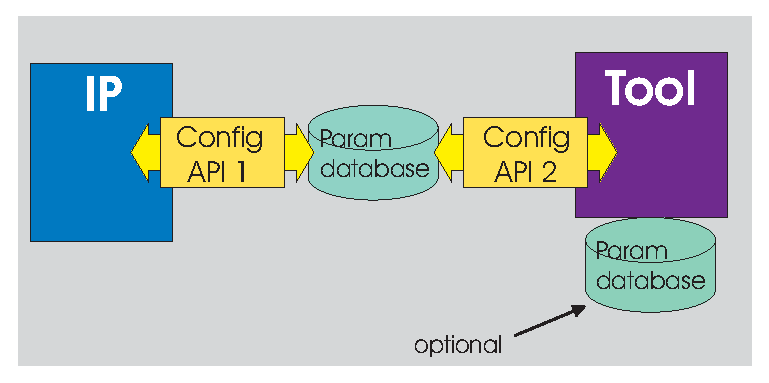
\includegraphics[width=10cm]{requirements_API_overview.eps}} 
	\caption{Overview configuration in general.}
	\label{fig:overviewAPIrequ}
\end{figure}



\subsection{Basic idea: the GreenConfig Core}
The \GreenConfig Core implements all functionality required to manage configurable parameters in SystemC models (implementation details follow below). It provides a generic GC-API which is used to built heterogeneous User APIs on top of it.  

Hence it has to be well designed to support virtually all functions other APIs might ask for. {\bf User API adaptors} translate between the \GreenConfig framework and the vendor's interfaces / APIs. 

\begin{figure}[H]%[htbp]
	\centerline{
		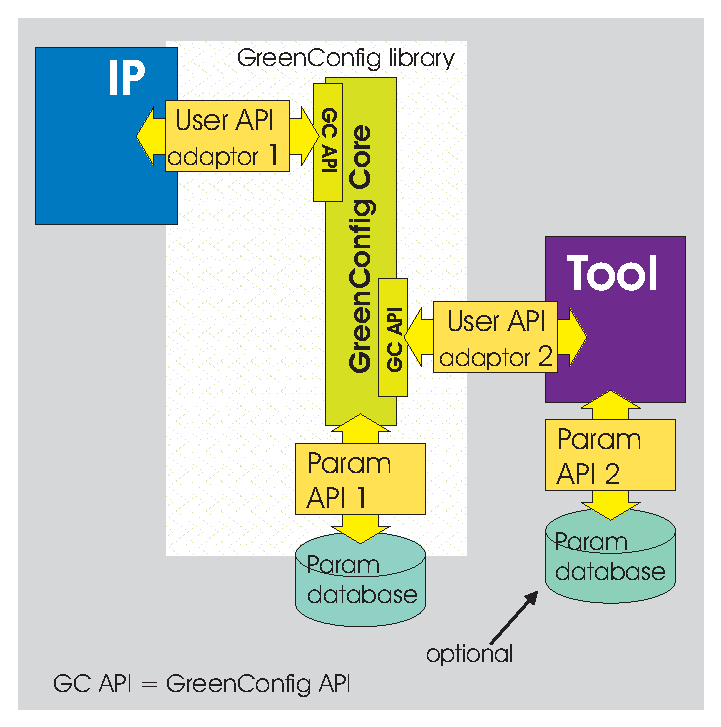
\includegraphics[width=10cm]{requirements_API_overview_GreenConfig.eps}} 
	\caption{Overview configuration with GreenConfig library.}
	\label{fig:overviewGreenConfrequ}
\end{figure}



\subsection{Main requirements}
\begin{itemize}
	\item Support {\em most} config APIs (as much as reasonable regarding effort) 
	\item Ease of use (i.e. usage requires minimal to no additional implementation effort) 
	\item Extensibility (e.g., support more data types, add new config file formats, add additional functionality) 
\end{itemize}



\subsection{Requirements classification}
We consider three classes of requirements: 

\begin{enumerate}
	\item Requirements for \GreenConfig to support known configuration APIs 
	\item Functionalities we from our point of view would like to see in \GreenConfig  
	\item Requirements for future directions 
\end{enumerate}



\subsubsection[(1.) Requirements to support other parameter configuration APIs]{(1.) Requirements for \GreenConfig to support other parameter configuration APIs}
\label{lab:requ1}
Table \ref{tbl:capabilitiesa} is based on the spreadsheet searching\_configurations\_in\_SystemC.xls 

These requirements (\ref{lab:requ1}) are made from the view of supporting the tool and user APIs of all other vendors. 

\begin{itemize}
	\item Provide an interface for the user and the tool (eventually uniform interface). This '\GreenConfig API' named interface is \GreenConfig internal and is used by the specialized 'User API adaptor' for a special vendor. The GC API has to support all thinkable functionality of any user and tool API of any vendor. 
	
	\item Interface to user API (\GreenConfig User API adaptor 1, see figure \ref{fig:overviewAPIrequ}) must allow: 
	
	\begin{itemize}
		\item Registering a parameter (The user can add a parameter to the configuration framework.) 
		\item Set default value (Set value of a parameter during elaboration) 
		\item Get value (Get the initial value of a parameter; set by default value or by tool) 
		\item Change value during runtime (The user may change value of a parameter even during simulation runtime.) 
		\item Notify changes to user (Register observer for a parameter either a parameter of the own module or a parameter of another module.) 
	\end{itemize}
	Interface to tool API (\GreenConfig User API adaptor 2, see figure \ref{fig:overviewAPIrequ}) must allow: 
	
	\begin{itemize}
		\item Configuration during elaboration / runtime (Set value of a parameter during elaboration and runtime) 
		\item Notify changes to tool (Register observer for a parameter which can be changed by the user during runtime) 
		\item Get value during elaboration / runtime (Get the value of a parameter during elaboration and runtime) 
		\item This interface may be used by a GUI tool 
	\end{itemize}

	\item The User API adaptors must be specialized for each vendor, using the \GreenConfig API and providing the vendor's APIs. 
\end{itemize}

\begin{landscape}
\begin{table}[H]
	\begin{tabularx}{23cm}{|X|X|X|X|X|X|}
		\cline{1-1}\cline{2-2}\cline{3-3}\cline{4-4}\cline{5-5}\cline{6-6}
		               & \multicolumn{5}{|l|}{ supported by    }\\ 
		\cline{1-1}\cline{2-2}\cline{3-3}\cline{4-4}\cline{5-5}\cline{6-6}
		               & {\bf Co\lstinline||Ware}   & {\bf ARM}   & {\bf TI} \newline no parameters   & {\bf Intel}   & {\bf GreenS. Simple \newline Config. \newline  Framew.}  \\ 
	
		\cline{1-1}\cline{2-2}\cline{3-3}\cline{4-4}\cline{5-5}\cline{6-6}
		Data types     & int, unsigned int, \newline double, bool, std::string    & std::string    & unknown, however \href{http://www.greensocs.com/SystemC/SystemCEvents/DATE2007Slides?action=AttachFile\&do=get\&target=systemPython-date-presentation-07.ppt}{presentation}  \newline implies that strings and  \newline number formats are supported   & "Instrumented Datatype" \newline user implemented \newline implement interfaces   & PODs, STL, SystemC  \\ 
		\cline{1-1}\cline{2-2}\cline{3-3}\cline{4-4}\cline{5-5}\cline{6-6}
		User defined types   & -   & yes (user implemented)   &     & yes (instrumented data type)   & yes (template specialized)  \\ 
		\cline{1-1}\cline{2-2}\cline{3-3}\cline{4-4}\cline{5-5}\cline{6-6}
		Permanent storage    & XML   & -   & -   & file   & file  \\ 
		\cline{1-1}\cline{2-2}\cline{3-3}\cline{4-4}\cline{5-5}\cline{6-6}
		Registering a parameter   & yes (global registry)   &  yes    &  -    &  drf module finds  \newline parameters itself   & yes (\lstinline|addParam| or macro \lstinline|GB_PARAM|  \\ 
		\cline{1-1}\cline{2-2}\cline{3-3}\cline{4-4}\cline{5-5}\cline{6-6}
		Set default value        & yes (constructor)   & user may implement   & user may implement   & yes   & yes (constructor)  \\ 
		\cline{1-1}\cline{2-2}\cline{3-3}\cline{4-4}\cline{5-5}\cline{6-6}
		Get value   & yes (e.g. \lstinline|getIntProperty(key)|   & yes (\lstinline|getParameter| \newline \lstinline|(string key)|)   & yes (pushed by method call)   & yes (Interface I\_dr\_dump)   & yes (\lstinline|get|)  \\ 
		\cline{1-1}\cline{2-2}\cline{3-3}\cline{4-4}\cline{5-5}\cline{6-6}
		Config. during runtime \newline Done by other module or tool   & -   & -   & yes (task\_start)   & -   & yes (\lstinline|set|)  \\ 
		\cline{1-1}\cline{2-2}\cline{3-3}\cline{4-4}\cline{5-5}\cline{6-6}
		Change value during runtime \newline Done by module itself   & yes   & yes (user implemented)   & yes (user implemented)   & yes (user implemented)   & yes (\lstinline|set| or direct)  \\ 
		\cline{1-1}\cline{2-2}\cline{3-3}\cline{4-4}\cline{5-5}\cline{6-6}
	\end{tabularx}
	\caption{(a) This spreadsheet shows the capabilities of the reviewed configuration systems.}
	\label{tbl:capabilitiesa}
\end{table}

\begin{table}[H]
	\begin{tabularx}{23cm}{|X|X|X|X|X|X|}
		\cline{1-1}\cline{2-2}\cline{3-3}\cline{4-4}\cline{5-5}\cline{6-6}
		               & \multicolumn{5}{|l|}{ supported by    }\\ 
		\cline{1-1}\cline{2-2}\cline{3-3}\cline{4-4}\cline{5-5}\cline{6-6}
		               & {\bf Co\lstinline||Ware}   & {\bf ARM}   & {\bf TI} \newline no parameters   & {\bf Intel}   & {\bf GreenS. Simple \newline Config. \newline  Framew.}  \\ 
	
		\cline{1-1}\cline{2-2}\cline{3-3}\cline{4-4}\cline{5-5}\cline{6-6}
		Notify changes to user   & -   & -   & yes (task call)   & yes (event as member of instr. datatype)   & -  \\ 
		\cline{1-1}\cline{2-2}\cline{3-3}\cline{4-4}\cline{5-5}\cline{6-6}
		Configuration during elaboration   & yes (instantiation, with global registry)   & yes (in user module \lstinline|setParameter(string| \newline \lstinline|key, string value)|)   & no (but task\_start)   & yes (Interface I\_dr\_config)   & yes (constructor or \lstinline|set|)  \\ 
		\cline{1-1}\cline{2-2}\cline{3-3}\cline{4-4}\cline{5-5}\cline{6-6}
		 / runtime   & -   & -   & method calls   & -   & yes (\lstinline|set|)  \\ 
		\cline{1-1}\cline{2-2}\cline{3-3}\cline{4-4}\cline{5-5}\cline{6-6}
		Notify changes to tool   & -   & -   & task-finished event   & -   & -  \\ 
		\cline{1-1}\cline{2-2}\cline{3-3}\cline{4-4}\cline{5-5}\cline{6-6}
		Get value during elaboration    & -   & -   & -   & yes (dump)   & -  \\ 
		\cline{1-1}\cline{2-2}\cline{3-3}\cline{4-4}\cline{5-5}\cline{6-6}
		 / runtime   & -   & -   & -   & yes (dump)   & -  \\ 
		\hline
	\end{tabularx}
	\caption{(b) This spreadsheet shows the capabilities of the reviewed configuration systems.}
	\label{tbl:capabilitiesb}
\end{table}
\end{landscape}




\subsubsection{(2.) Requirements for GreenConfig in General from bottom-up}
\label{lab:requ2}
These requirements describe the framework from our view without regarding special other APIs but to achieve a many-sided framework. 

\begin{enumerate}
	\item {\em Usage} 
	\begin{enumerate}
		\item New datatypes can be easily added by the user (to provide as many datatypes as possible) 
		\begin{enumerate}
			\item Methods to set and get the value of the parameter use \lstinline|std::string|: \newline  void set(const std::string \&str) and const std::string get()  \newline  This allows easy adaption of the tools to set a parameter and is universal. 
			\item The data type of a template should be given as template parameter.  \item Usage of a templated parameter (\lstinline|gs_param<datatype>|) should be as easy as the usage of the data type itself by overloading the operators (\&, =). This is the instrumentation of a member variable to use it as a parameter. The usage of the parameter is transparent due to the overloaded operators. (SOW 3.1.3) 
		\end{enumerate}
		\item Support all imaginable parameter types and usages, e.g. 
		\begin{itemize}
			\item Setup parameters: Setup parameter is set during elaboration. The module complies with the value of the parameter to act variedly. 
			\item Change setup parameters: Parameter which changes during runtime to take influence on the behavior of the module. 
			\item Status parameters: Status parameter represent the status of a module. They are set by the module itself. Observers are notified when it changes. 
			\item Output parameters: Parameters to send output (debug values etc.) to the tool outside the simulation. 
			\item ... 
		\end{itemize}
	\end{enumerate}

	\item {\em Configuration} 
	\begin{enumerate}
		\item Configuration during elaboration 
		\item Configuration during runtime 
		\item Use same configuration system (same methods etc.) for initial configuration during elaboration and runtime configuration during simulation 
		\item Provide setting of parameters to other IPs (e.g. tools) 
		\begin{itemize}
			\item Setting of a parameter: \lstinline|setParameter(std::string hierarchical_name, std::string value)| 
		\end{itemize}
		\item Provide getting of parameter values to other IPs (e.g. tools) 
		\begin{itemize}
			\item Getting of a parameter value: \lstinline|std::string getParameter(std::string hierarchical_name)| 
		\end{itemize}
		\item Provide setting of parameters inside user code. There are two different types: 
		\begin{enumerate}
			\item Setting of the parameter in the module which contains the parameter: \newline Inside the parameter holding module the user may choose out of two ways of setting the value.  
			\begin{itemize}
				\item The user can set the value with the setting method (see requirement 1.1.1) using the parameter's string representation. 
				\item The value can be set with the instrumentation of the member variable by simply assigning the value (see requirement 1.1.3). 
			\end{itemize}
			\item Setting of the parameter of module in another module
						 We have two options to realize the access to parameters of another module: First we can access them directly by pointer. This assumes the availability of the pointer which has to be provided by a central unit. It is clearer to provide the setting of a parameter by a function contained in the API of the library. Here the same method can be used which is also used by the tool API to set parameters (see requirement 2.4). 
		\end{enumerate}
		\item A default value can be set during instantiation/construction of the parameter: \lstinline|gs_param(const char *name, T value)|. 
	\end{enumerate}

	\item {\em Core} 
	\begin{enumerate}
		\item Efficient data management (database) for runtime (how parameters are saved during runtime, e.g. map, list,...) 
		\item Efficient data management (database) for permanent storage (e.g. config file, XML file, Access database,...) 
		\item Find local and global identification system for parameters (names): Unique name inside module, full name composed of hierarchical names leading to parameter name (\lstinline|module_name.submodule_name.parameter_name|) 
		\begin{itemize}
			\item Name a parameter during instantiation with \lstinline|my_param = gs_param<datatype>(my_name)|. 
			\item Get the parameter name with \lstinline|const std::string &getName()|. 
		\end{itemize}
	\end{enumerate}

	\item {\em Observation / notification} 
	\begin{enumerate}
		\item Provide a complete parameter list: e.g. \lstinline|multimap<const char * hierarchical_prefix, const char * name> getParameterList()| or \lstinline|list<std::string hierarchical_name> getParameterList()| 
		\item Allow an observer to register for a parameter to be notified with an event when it changes 
		\begin{enumerate}
			\item Allow many observers per parameter 
			\item Additional one event per configurable module \lstinline|config_changed|? 
		\end{enumerate}
		\item Provide to the module itself an event which is notified when any parameter of the module is changed (function callback {\em and} sc\_event) (see requirement 4.2.2). 
		\item Either the parameters have to register themselves at the library or the library finds the parameters or modules due to the implementation of the config interface (e.g. \lstinline|gs_configurable|). 
	\end{enumerate}

	\item {\em Additional requirements resulting on conference call on 21st May 2007} 
	\begin{itemize}
		\item Secure IPs which allow disabling their configuration abilities. 
		\item Some kind of privacy tags to protect parameters being changes from outside the module. 
		\item Recording actions (who is when setting or getting etc.) in the Core 
	\end{itemize}

\end{enumerate}


\subsubsection{(3.) Requirements for the support of other control interfaces}
These requirements are formed by additional control issues. Here not the parameter configuration must be provided but more general control methods. E.g. configuration or starting a task with the call of a configuration method which is provided by a given or user defined interface . 

This part is for future use and has no priority at this moment. 

\subsection{Sorted and prioritized requirements}

\begin{enumerate}
	\item Default value during construction 
	\item Configuration during elaboration 
	\item Configuration during runtime (Callback/event on change) 
	\item Supported data types (set and get with strings, addition of parameter types easy) 
	\item User defined data types 
	\item Notify changes to tool (Callback/event on change) 
	\item Notify changes to user module (Callback/event on change) 
	\item Permanent storage in file 
\end{enumerate}


\end{document}
